\chapter{The CMS Detector}\label{chap:cms}


% \vspace{-5pt}
\section{Introduction}\label{sec:ch3:intro}

 \begin{figure}[h]
\centering
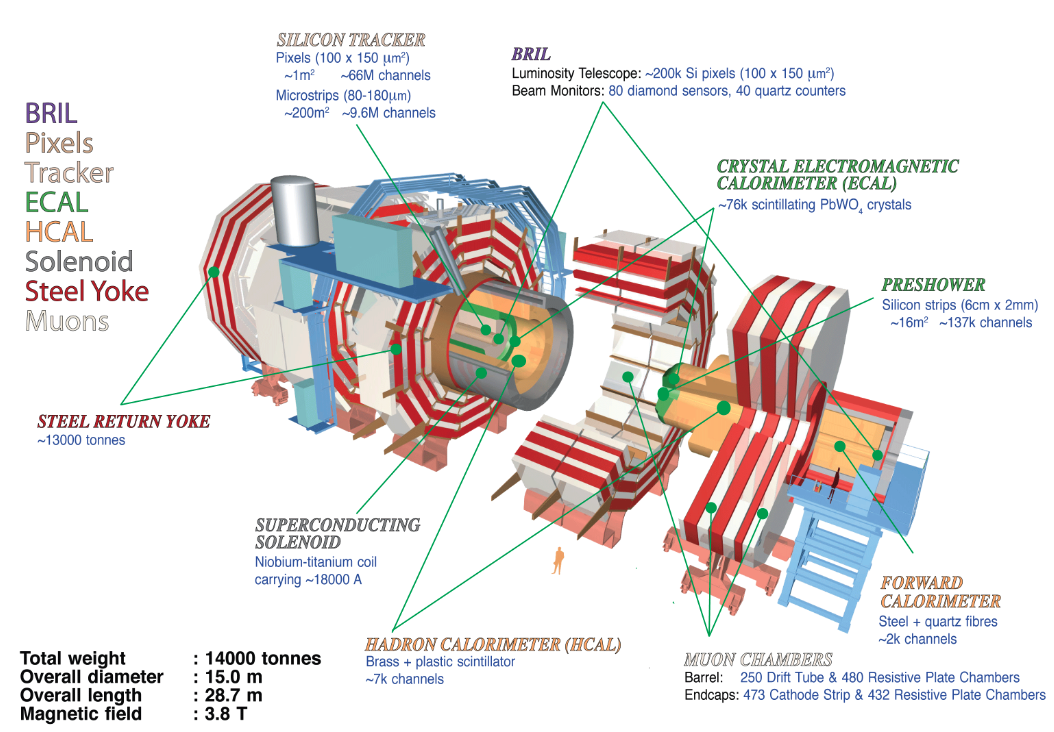
\includegraphics[width=0.8\textwidth]{figures/cms_schematic.png}
\caption{Schematic of the Compact Muon Solenoid (CMS) detector~\cite{cms_schematic}.}
\label{fig:cms}
\end{figure}

Figure \ref{fig:cms} shows the schematic of the Compact Muon Solenoid (CMS) detector. The detector is located in the Large Hadron Collider (LHC), which is depicted in the collider apparatus in Figure \ref{fig:cern}.

 \begin{figure}[h]
\centering
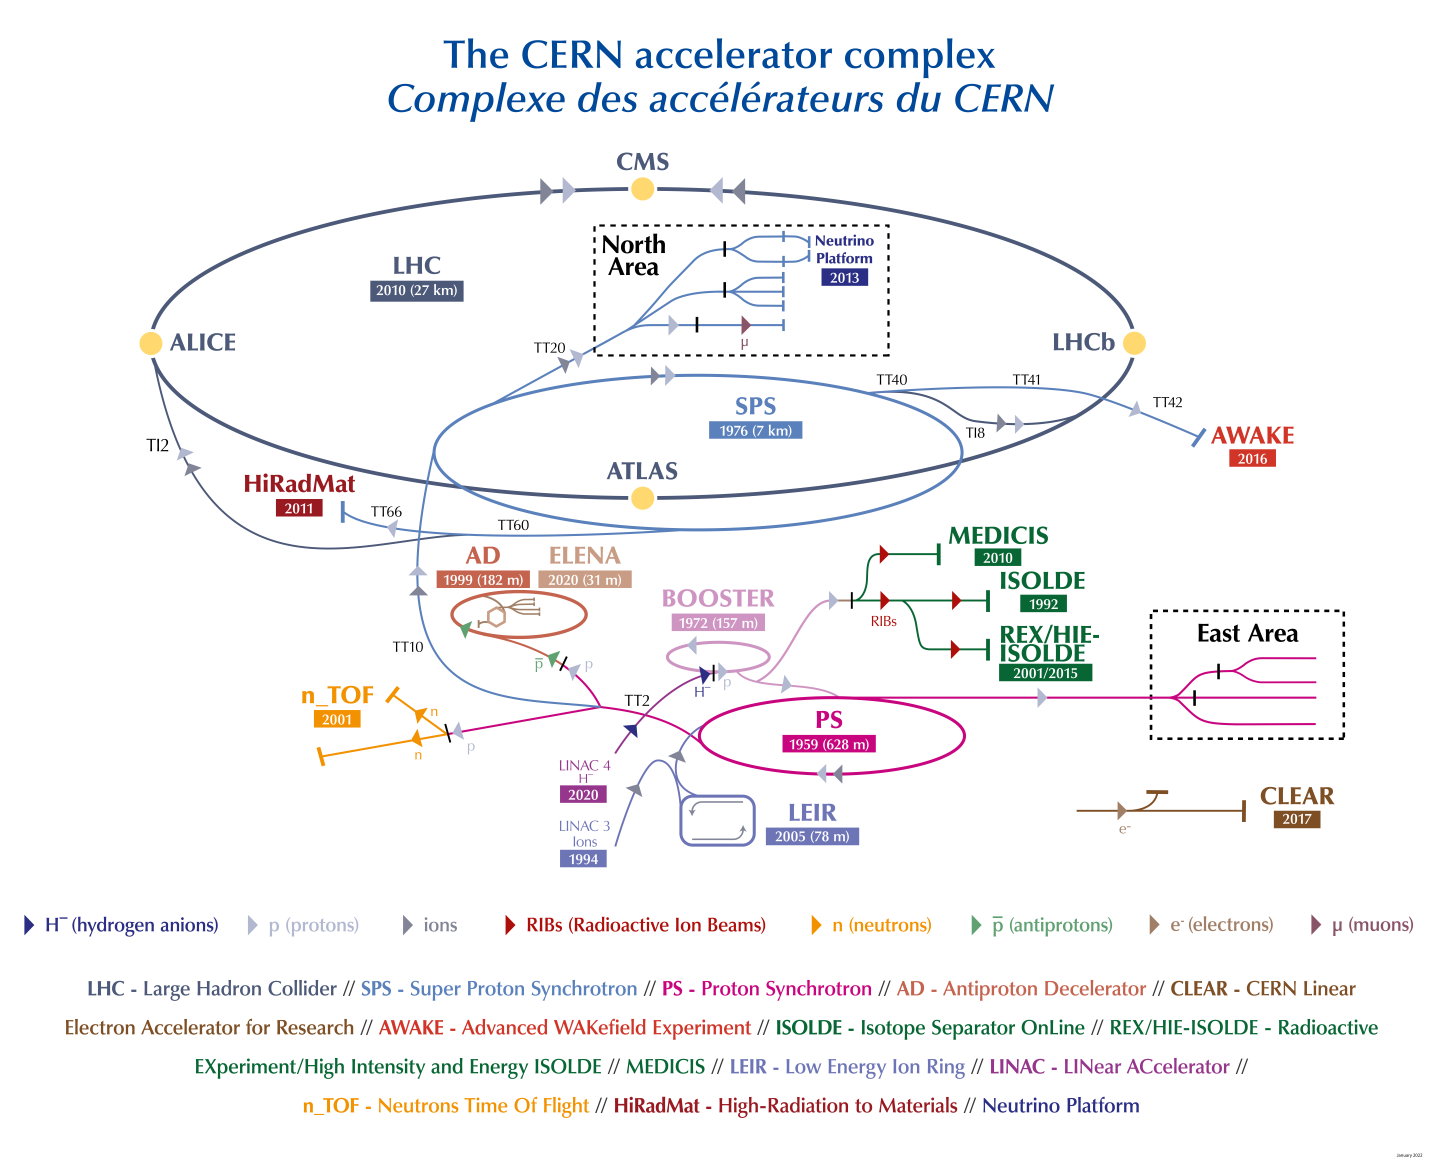
\includegraphics[width=1.0\textwidth]{figures/CCC-v2022.png}
\caption{Schematic of the collider apparatus at CERN~\cite{CERN_Accelerator_Complex}.}
\label{fig:cern}
\end{figure}


The Large Hadron Collider (LHC) beam energy, originally at 7 TeV, now for Run 3 at 13.6 TeV, allows us to study physics at the highest energy scale ever in a laboratory setting. The collaboration also performs studies of heavy ions at 30x the energy of previous heavy ion experiments. With a luminosity for pp collisions 100x greater than previous experiments, and pp cross section of about 100 mb, measurements can be done to greater precision than ever before, and searches can probe the highest ever possible masses at the TeV scale.

The LHC contains multiple experiments. At opposite points of the collider, 27 km apart, sit ATLAS (or the experiment formerly known as A ToroidaL ApparatuS) and the Compact Muon Solenoid (CMS) experiments. The experiments perform similar searches and measurements without sharing preliminary results. This mitigates biases from experimentalists during the analyses.

The CMS detector is located at Point 5 at the Large Hadron Collider~\cite{CMSExperiment}. It has several subsystems, including the tracker, the electromagnetic calorimeter, the hadronic calorimeter, the solenoid, and the muon chambers. The CMS detector is cylindrical and so each detector has a cylindrical "barrel" region and disk-shaped "endcap" region. The Endcap regions are necessary as nearly $1/3$ of all particles cross the $1.3 < |\eta| < 3$ region.

\vspace{-3pt}
\section{The Tracker}\label{sec:ch3:trk}


\begin{figure}[h]
\centering
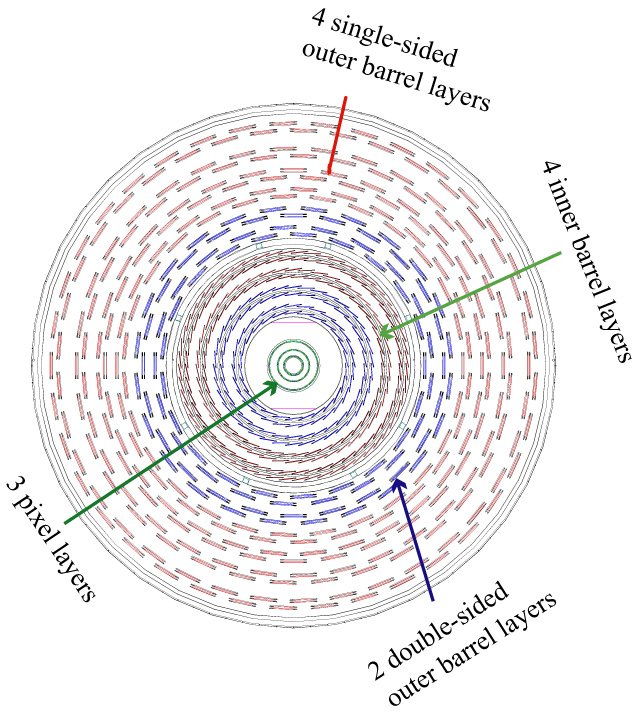
\includegraphics[width=0.5\textwidth]{figures/Barrel_0_tracker.png}
\caption{Schematic of the tracker.}
\label{fig:tracker_circular_schematic}
\end{figure}

 \begin{figure}[h]
\centering
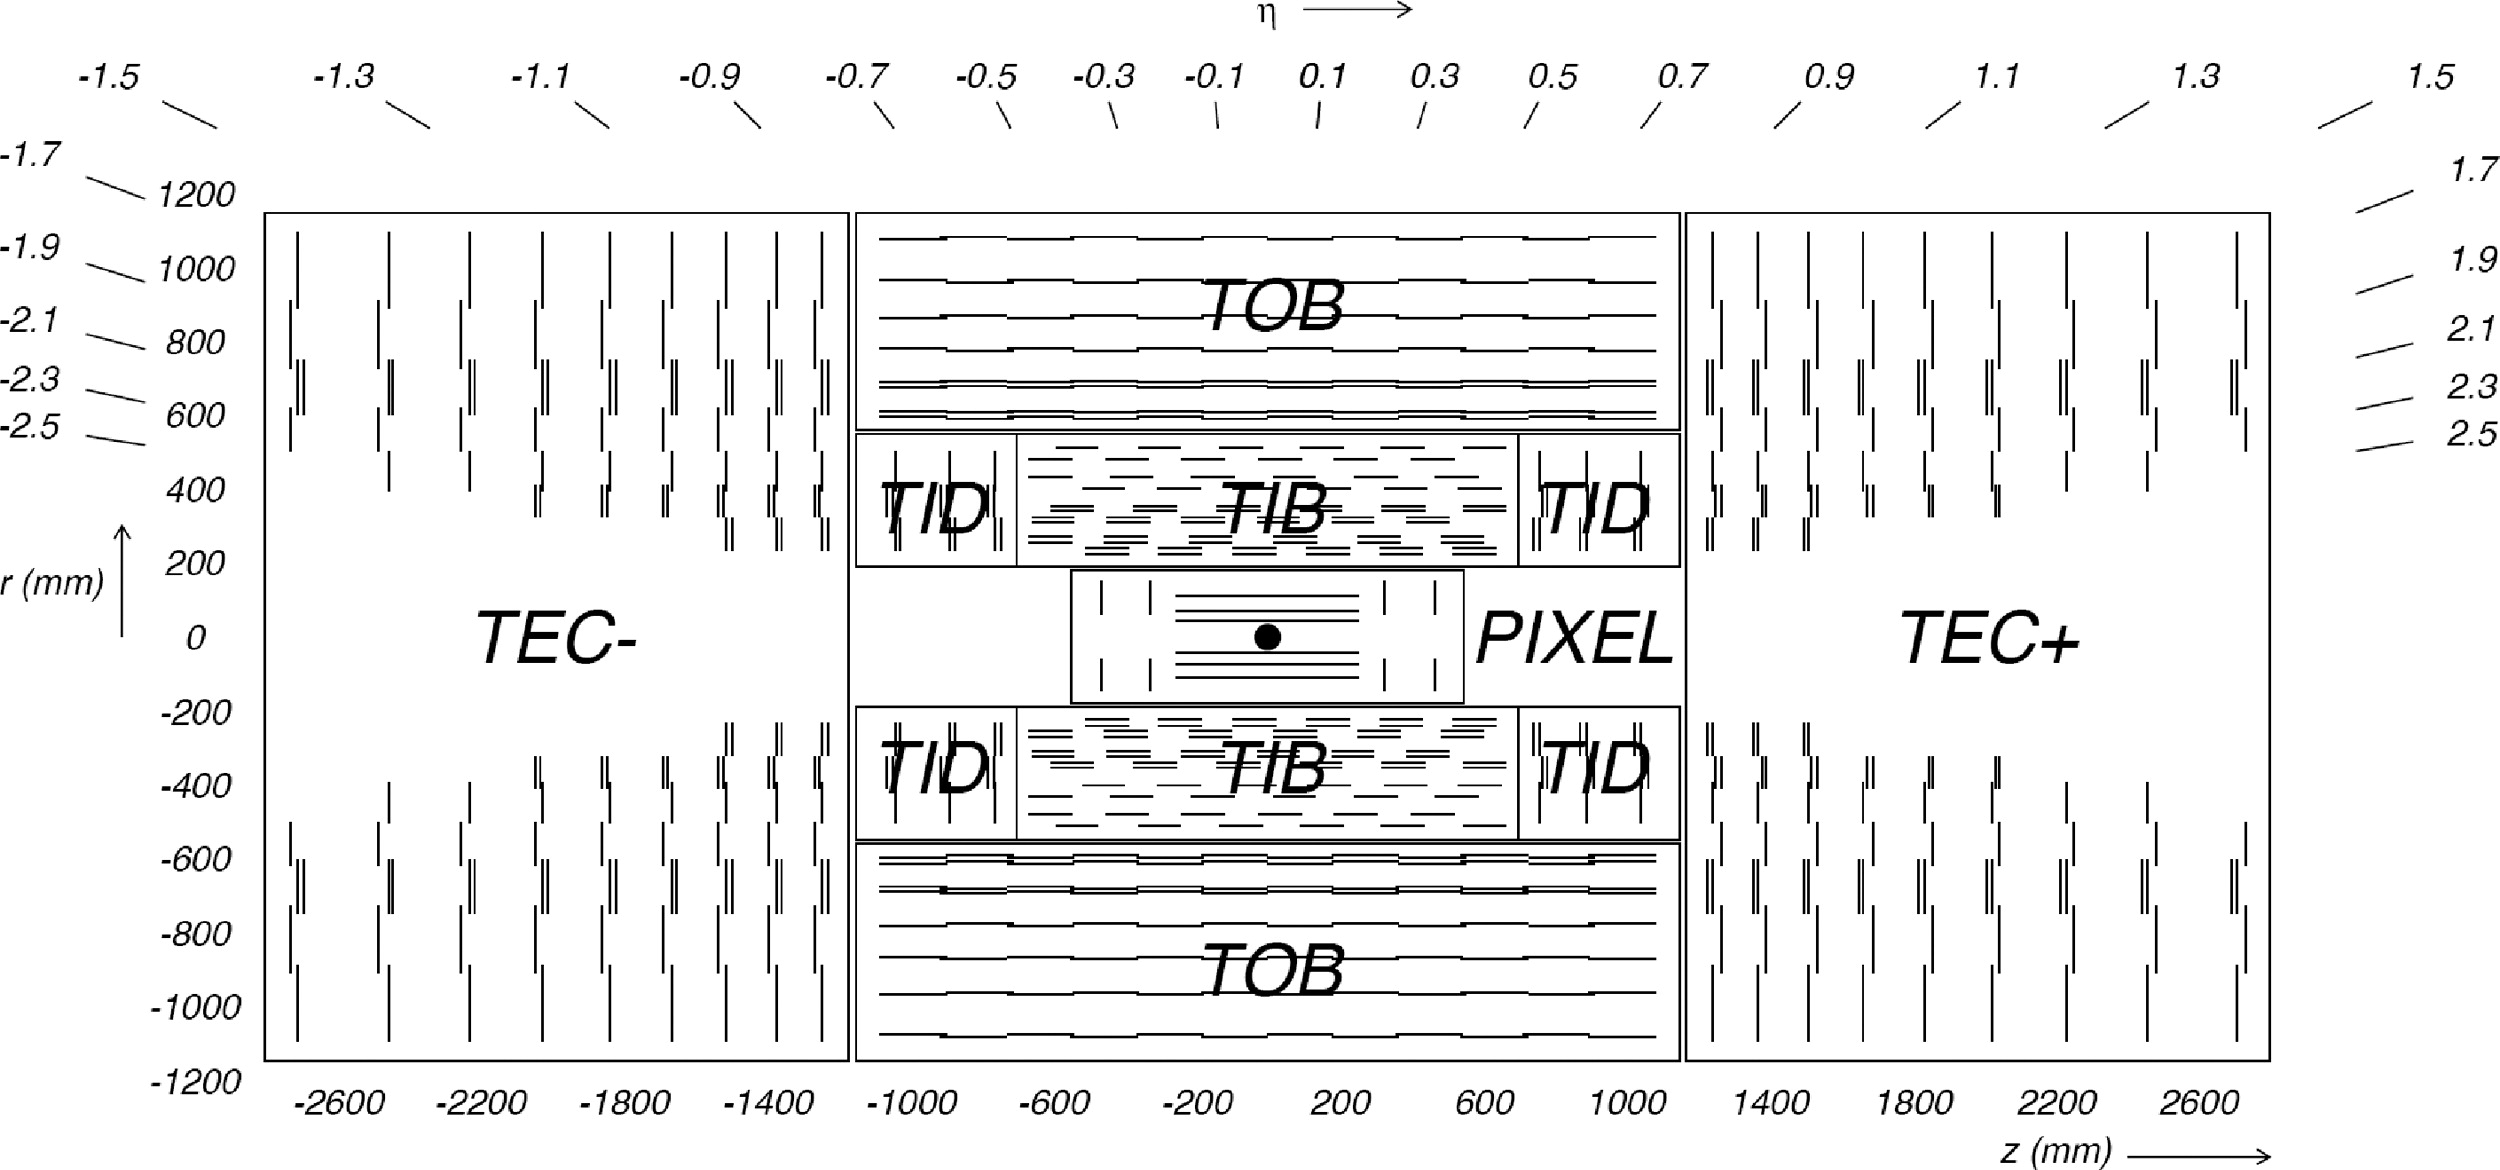
\includegraphics[width=1.0\textwidth]{figures/cms_tracker_cross_section_schematic.jpg}
\caption{Schematic of the tracker, projected onto an $z$-$r$ plane.}
\label{fig:cms_tracker_cross_section_schematic}
\end{figure}

At the innermost layer of the detector, held within the 6 meter bore of the solenoid, sits the silicon tracking system. With 1000 particles from 20 overlapping collisions bombarding the detector every 25 ns, the tracker needs a high power density system to accurately and precisely measure the tracks of individual charged particles. The high energy particles subject the electronics to high radiation levels. A radiation-hard material cooled to low temperatures is needed to withstand these high levels. For this, silicon was used, and has tracker has been operating for over a decade, longer than the planned lifetime of the detector. The tracker was built over the course of over a decade, with the input of hundreds of particle physicists from 51 institutes, including the University at Buffalo.


The tracker is composed of two subdetectors: an inner 3-layer pixel detector pixel detector and an outer 10-layer strips detector. inner , with 10 barrel layers of silicon strip tracking. In Figure~\ref{fig:tracker_circular_schematic}, the positions of these layers are shown on a circular cross-section of the cylindrical Tracker. Inside the innermost circle is the beam line where the interaction point for the detector sits. This interaction point is depicted as a black dot in Figure~\ref{fig:cms_tracker_cross_section_schematic}, which shows the detector projected onto an $r$, $z$ plane.  The 3 barrel layers of the pixel detector are the 3 lines above and below the interaction point. The pixel barrel (BPix) is 53 cm long with the largest radius at 10.2 cm, which allows coverage of $|\eta| > 2.5$. The pixel front endcaps (FPix) are position in 2 layers at $|z| = 34.5$ cm and $|z| = 46.5$ cm. The pixel layers have high granularity to allow for precise measurement of the position of the detected particles. Each pixel has an area of $100x150$ \textmu m, with 48 million pixels in BPix and 18 million in FPix~\cite{CMSExperiment}.

The strip tracker surrounds the pixel subdetector. In Figure~\ref{fig:cms_tracker_cross_section_schematic}, the subdetectors for the strips tracker are shown. The tracker inner barrel (TIB) has 4 layers with 320 \textmu m thick silicon strip sensors. The tracker outer barrel (TOB) has 6 layers with 500 \textmu m thick silicon strip sensors. The tracker has disk layers covering the high $|\eta|$ region. The tracker inner disks (TID) have 3 layers, and the tracker endcaps (TEC) have 8 layers. The TEC, TID, and FPix disk layers and the TOB, TIB, and Bpix barrel layers supply a total of 22 measurements with resolutions ranging from 23 \textmu m to 53 \textmu m, further described in Table~\ref{tab:rphi_mmts}.

\begin{figure}[h]
\centering
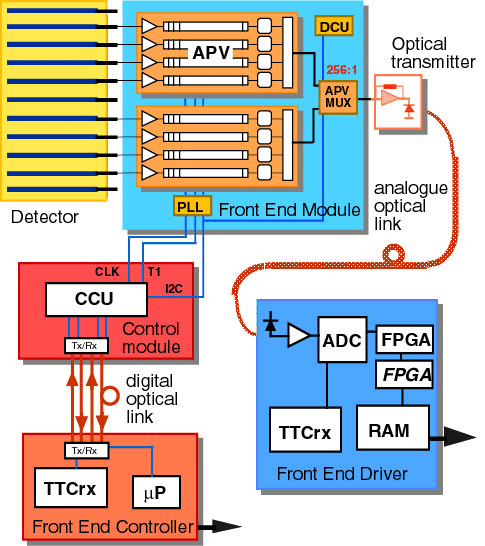
\includegraphics[width=0.5\textwidth]{figures/Read-out-scheme-of-the-CMS-Tracker.png}
\caption{Schematic of the tracker readout system~\cite{CMSExperiment}.} \label{fig:tracker_readout}
\end{figure}

\begin{table}
\begin{center}
\begin{tabular}{||c c c||} 
 \hline
 Subdetector & Resolution & $r-\phi$ Measurments \\ [0.5ex] 
 \hline\hline
 BPix/FPix &  & 3 \\ 
 \hline
 TIB/TID & 23-25 \textmu m & 4 \\
 \hline
 TOB & 35-53 \textmu m  & 6 \\
 \hline
 TEC &  & 9 \\ [1ex] 
 \hline
\end{tabular}
\caption{Resolution of the pixel and strips subdetectors with the number of measurements in $r-\phi$ each supplies~\cite{CMSExperiment}.}
\label{tab:rphi_mmts}
\end{center}
\end{table}
%
%\begin{todolist}
%	\item describe silicon strip sensors
%\end{todolist}


The tracker materials must be kept to low temperatures to mitigate the damage caused by the radiation from the beam collisions. Cooling liquid is transported to the silicon sensors by aluminum pipes, which are formed into cooling loops and attached to the sensors with aluminum ledges.

The information from the silicon sensor is sent through a readout system, shown in Figure~\ref{fig:tracker_readout}. Fiber optic cables carry analog signals from the sensors in the tracker to Front End Drivers (FEDs). The FEDs convert the analog signals to digital. Front End Controllers (FECs) transmit signals from the clock, control systems, and trigger. The information from the tracker is vital to the high level trigger (HLT) decisions, which reduce the rate of incoming collisions data by a factor of 400. Silicon modules contain either one of the 320 \textmu m or 2 of the 500 \textmu m thick silicon sensors. The modules are grouped into power groups that are each powered by one power supply, which supplies 2 low voltage lines at 1.25 V and 2.5 V, and 2 high voltage lines. The silicon sensors are made of p-on-n type material. On the back, n type aluminum is used to connect to a positive voltage. On the other side are the p+ type silicon strip diodes. 

The Detector Control Systems (DCS) are designed using a Supervising Control and Data Acquisition (SCADA) program developed with WinCCOA. The DCS is a Final State Machine tree that controls all of the power supplies. A Detector Control Unit monitors the low voltage, leakage current, and temperature of the silicon sensors.

The radiation length of materials used in the tracker shown in Figure~\ref{fig:tracker_radiation_length.}.

\begin{figure}[h]
\centering
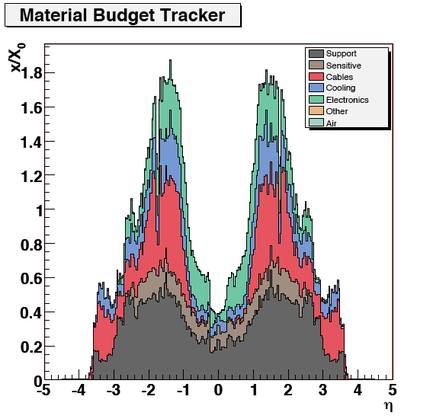
\includegraphics[width=0.5\textwidth]{figures/tracker_radiation_length_XoverX0.png}
\caption{Radiation length of materials used in the tracker~\cite{CMSExperiment}.}
\label{fig:tracker_radiation_length.}
\end{figure}



\vspace{-3pt}
\section{The Electromagnetic Calorimeter}\label{sec:ch3:ecal}

The Electromagnetic Calorimeter (ECAL) surrounds the tracker. Its purpose is to absorb the energy from electrons and photons, and was built with the motivation of detecting the decay of two photons for Higgs boson searches. The ECAL is composed of thousands of lead tungstate (PbWO$_4$) crystals, which are mounted on a barrel layer and two endcaps. Before the endcaps, a preshower made of two planes of lead reduces false signals.

Lead tungstate crystals are useful in a compact detector because they are radiation-hard and have a small radiation length and small Moliere radius. Additionally, the scintillation decay time of lead tungstate is approximately 25ns, which is the same as the bunch crossing separation in the LHC. The barrel receives the particle data through avalanche photodiodes, which apply a reverse bias voltage to get a current gain effect of about 50. The endcaps use vacuum phototriodes, which are photomultipliers with a single gain state. The vacuum phototriodes usee in the ECAL were developed specifically for CMS, and are useful in the endcaps because they are more radiation resistant than diodes.

The barrel of the ECAL covers $|\eta| < 1.479$, and the endcaps cover $1.479 < |\eta| < 3.0 $. Water cools the submodules containing the crystals at a temperature of 18$^{\circ}$C.


The energy resolution in the ECAL is described by Equation \ref{eq:ecal1}.

\begin{equation}
\left( \frac{\sigma}{E} \right)^2 = \left( \frac{S}{\sqrt{E}} + \left( \frac{N}{E} \right)^2\right)^2 + C^2
\label{eq:ecal1}
\end{equation}

$S$ is the stochastic term, and is comprised of photostatistics (about 2.1\%), fluctuations in energy deposited in the preshower (about 5\%/$\sqrt{E}$), and fluctuations in the lateral shower containment (about 1.5\%). $N$ is the noise term, and is comprised of electronics, digitization, and pileup noise. $C$ is the constant term, and is made up of leakage from the back of the crystals, intercalibration errors, and non-uniformity in light collection, the last being less than a 0.3\% contribution.

\vspace{-3pt}
\section{The Hadron Calorimeter}\label{sec:ch3:hcal}

\begin{figure}[h]
\centering
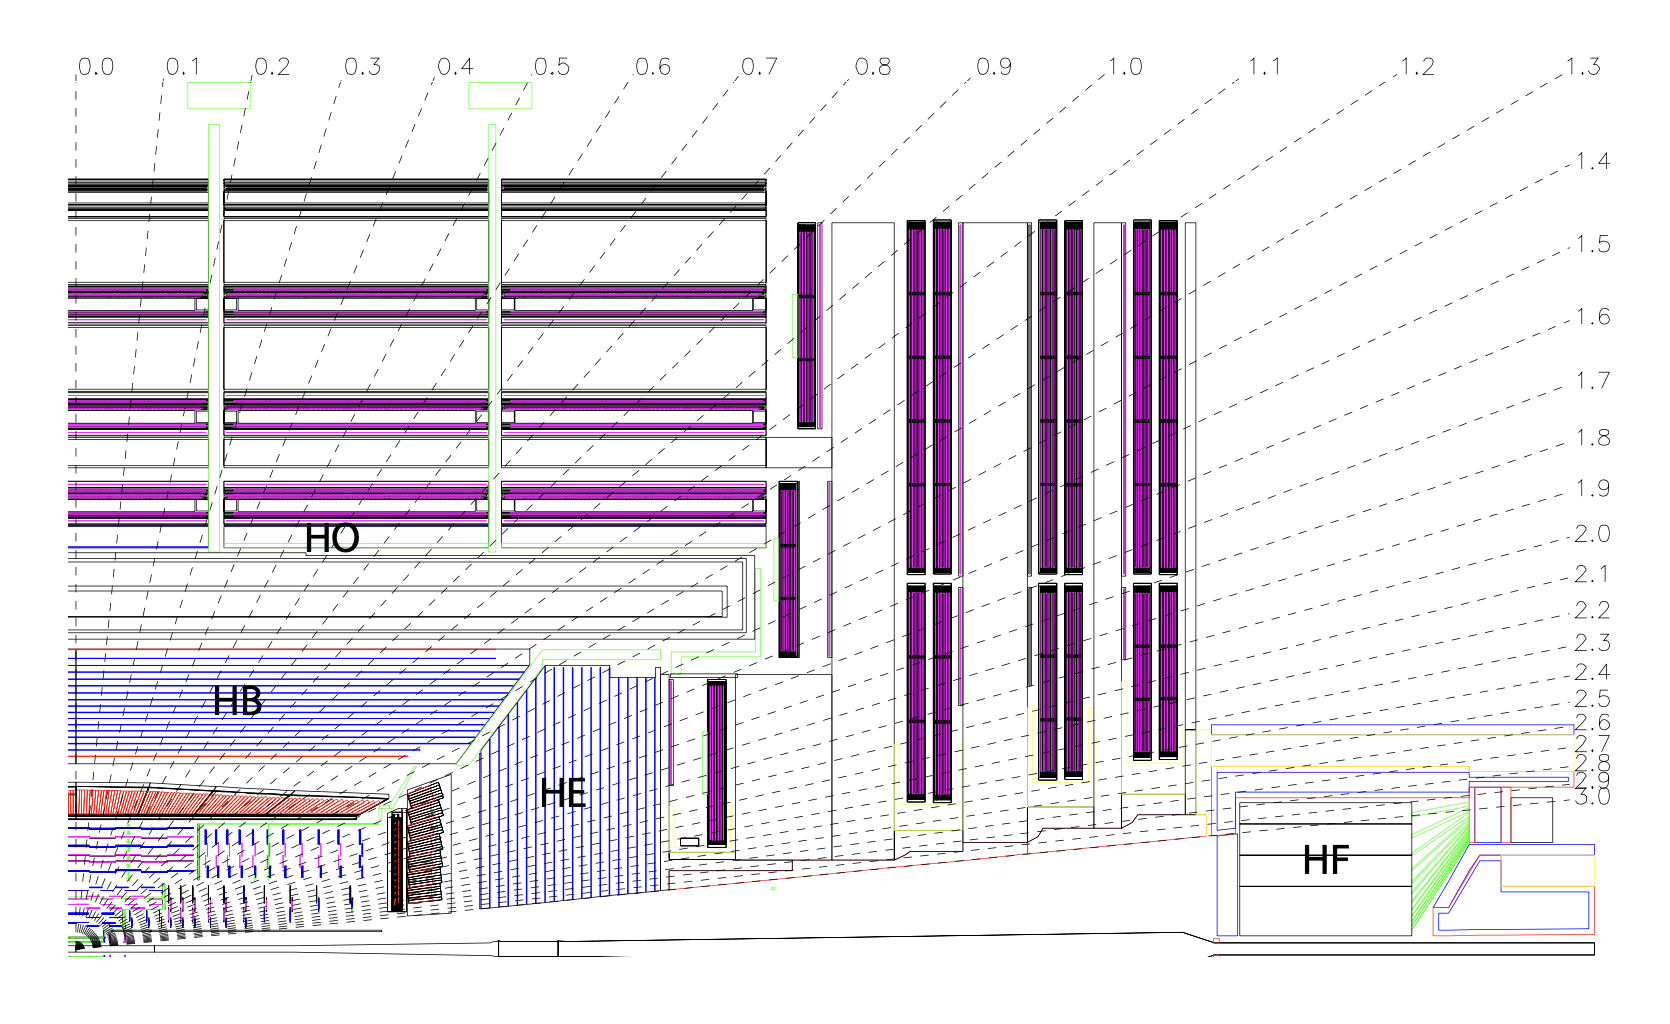
\includegraphics[width=1.0\textwidth]{figures/HCAL.png}
\caption{Schematic of the Hadron Calorimeter.}
\label{fig:HCAL}
\end{figure}


\begin{figure}[h]
\centering
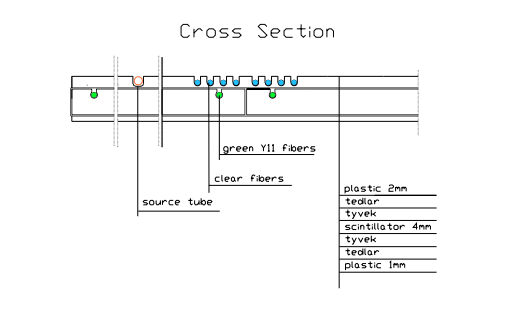
\includegraphics[width=1.0\textwidth]{figures/hcal_scintillator_replace.png}
\caption{Schematic of the plastic scintillator in the HCAL.}
\label{fig:HCAL_scint}
\end{figure}

The Hadron Calorimeter (HCAL) is designed to absorb the energy from the hadronic particles. It is split in four sections: the barrel (HB), the endcap (HE), the outer calorimeter (HO), and the forward calorimeter (HF), shown in Figure~\ref{fig:HCAL}. The barrel (HB), covers $|\eta| < 1.3$, and the endcaps (HE), cover $1.3 < |\eta| < 3.0$. The HB is a sampling calorimeter of absorber (bronze) and scintillator (plastic). The brass absorber is divided into 36 wedges in $\phi$. The plastic scintillator is divided into 16 sectors in $\eta$. The brass absorber is used for it's cost, radiation hardness, and non-magnetic properties.

The HCAL has a limited distance between the ECAL and the solenoid to absorb the hadronic particles. For particles that are unable to be stopped in that distance, an outer calorimeter is placed outside the solenoid in the central eta region



Hadrons penetrate more material than electrons and photons. Some hadrons still are not completely absorbed by the HCAL subdetectors between the ECAL and solenoid. Therefore the HO is set outside of the solenoid at R = 4.07 to catch any hadrons that are not stopped by the HB or HE. The HB is a sampling calorimeter with alternating layers of brass absorber and plastic scintillator. The brass absorber plates in the HB are positioned parallel to the beam line in a staggered formation. The first and last layer of the HB is a steel to serve as both an absorber layer and to provide structural strength. The HB has a total absorber length of 5.82 $\lambda_I$, where $\lambda_I$ is the interaction length of hadronic particles. The interaction length increases with $\theta$ as $1/\sin{\theta}$, for an thickness of 5.82 $\lambda_I$ at the edge of the HB at $|\eta| = 1.3$.

The scintillators are made of the material Kuraray SCSN81, which is a stable and radiation hard plastic. The plastic is formed into 70,000 tiles which are layered in trays between the brass absorber plates. One layer plastic scintillator sits in front of the steel absorber and one behind to catch any showers that start before the HCAL or that leak out the start of the HCAL. Tubes carry radioactive material through the plastic scintillator tiles for Cs$^{137}$ for calibration. A schematic of the plastic scintillator is shown in Figure~\ref{fig:HCAL_scint}.

The plastic scintillators detect the hadrons which are stopped by the brass absorbers. When a hadronic particle enters the plastic scintillator, the photoelectrons ionize and experience a gain of 2000 in the diode. Fiber optic cables in the scintillator carry the light to clear fiber. optic cables which carry the light to the photodiode. A diagram of a generic scintillator is shown in Figure~\ref{fig:scintillator}.

\begin{figure}[h]
\centering
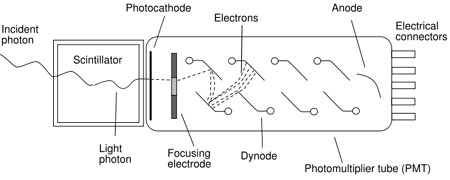
\includegraphics[width=1.0\textwidth]{figures/scintillator.jpg}
\caption{A scintillator converting an incoming photon to an electric signal.}
\label{fig:scintillator}
\end{figure}

The HB covers a pseudorapidity range of $|\eta| < 1.3$. The HE covers the range of $1.3 < |\eta| < 3$. The HE is also made of an alternating brass absorber and plastic scintillator. The HE covers 10 $\lambda_I$.

The solenoid also acts as an absorber with an interaction length of $1.4/\sin{\theta}$. Any hadrons that still have not been completely absorbed will then enter the outer HCAL (HO). With the HO, HB, and HE, the HCAL has a total absorption of 11.8 $\lambda_I$, with drops in efficiency only where the borders of the subdetectors meet.

The HF is made entirely of steel absorber with no scintillator between The HF is a thickness of 165 cm which corresponds to 10 $\lambda_I$ in steel. Electrons and photons will be absorbed within the first.
The Large Hadron Collider (LHC) beam energy, originally at 7 TeV, now for Run 3 at 13.6 TeV, allows us to study physics at the highest energy scale in history. The collaboration also performs studies of heavy ions at 30x the energy of previous heavy ion experiments. With a luminosity for pp collisions 100x greater than previous experiments, and pp cross section of about 100 mb, measurements can be done to greater precision than ever before, and searches can probe the highest ever possible masses at the TeV scale.

The LHC contains multiple experiments. At opposite points of the collider, 27 km apart, sit the A ToroidaL ApparatuS (ATLAS) and Compact Muon Solenoid (CMS) experiments. The experiments perform similar searches and measurements without sharing preliminary results. This ensures a mitigation of biases from persons performing the analyses.

The CMS experiment has 5 layers. From innermost to outermost layer sits the tracker, the electromagnetic calorimeter, the hadronic calorimeter, the solenoid, and the muon chambers. The solenoid has a 4T magnetic field. It is 13 meters long with a 6 meter inner diameter. To keep the solenoid compact, the coil is wound 4 times over to generate the 4T magnetic field. The 4T field requires a large return yoke, and so 6 endcaps and 5 barrel wheels, weighing up to 1920 tons, make up the yoke. In order to slide the solenoid in and out of the detector, the solenoid is placed on a system of air pads and grease pads that can slide the solenoid a total of 11 meters into or out of the detector. The process of sliding the solenoid 11 meters takes 1 hour to complete.

The superconducting solenoid needs to be cooled to temperatures between 4.5K and 80K. To do this, liquid helium is used and the solenoid is insulated with a 40 m$^3$ vacuum chamber. The solenoid is built to withstand a misalignment up to 10 mm between the coils and the return yoke.

The CMS solenoid is 13m long with a 6m bore diameter. The tracker, ECAL, and HCAL are situated within the bore. Due to the number of turns needed to generate a 4T magnetic field, and due to the compact nature of CMS, the solenoid is wound in 4 layers.


\vspace{-3pt}
\section{The Muon Detector System}\label{sec:ch3:muon}

\begin{figure}[h]
\centering
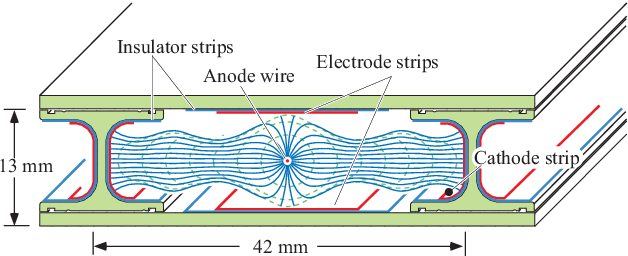
\includegraphics[width=0.75\textwidth]{figures/muon_DT_schematic.png}
\caption{Schematic of a muon detector drift tube~\cite{drift_tube_image}.}
\label{fig:muon_DT_schematic}
\end{figure}


The muon detector system is what gives the Compact Muon Solenoid detector its name. Muons are one of the most difficult standard model particles to detect, as their radiation lengths are often much longer than the length of a detector. In addition to the difficulty of detecting muons originating from collision events (called "prompt" muons), cosmic ray muons originating from our sun bombard the earth at very high rates. A muon detector system must then be very sensitive to muons while being highly shielded from cosmic rays. While some particles that are not muons may make it through the 16 $\lambda_I$ of the Tracker, ECAL, HCAL, and solenoid, the rate is so low that these hits in the muon detector are considered negligible.

Since muons experience little radiative loss in the detector, their 4-momentum can be reconstructed with high accuracy. At low momenta of $p_T < 200$ GeV, the momentum resolution is 9\%. For $p_T 1000$ GeV, the momentum resolution increases to 40\%. Together, the barrel and endcaps can trigger on the $p_T$ of muons without any extra information from the other detectors. At the Level 1 trigger, the resolution of the muons is 15-25\%.

 The barrel of the muon detector system is made of drift tube cells with 2 parallel electrode strips with a gold plate anode wire through the center of the cell also parallel to the electrode plates. A schematic of a muon drift tube is shown in Figure~\ref{fig:muon_DT_schematic}. The drift tube is filled with an AR-CO$_2$ gas mixture that provides a gain of $10^5$. 
 
 The drift tubes are staggered with an offset of 1/2 the length of a drift tube cell The staggering also helps with the detection of background hits that do not correspond to a detected track. The staggering allows the paths from muons to be reconstructed using hits from different drift tube cells.

The endcaps receive a higher rate of muons. The endcaps cover the pseudorapidity range $0.9 < |\eta| < 2.4$ and are made of Cathode Strip Chambers (CSC). Since the barrel covers the range $|\eta| < 1.2$, there are no gaps in the muon detector coverage for $|\eta| < 2.4$. 





